\section{Team constellation}
\label{ProjMgmtTeams}
This section explains the team environments in which the project takes place. This serves to provide an understanding of the direct project team working on this project and other teams at Swiss Post that contribute to the goals of the project.

\subsection*{Relevant Swiss Post teams}

At Swiss Post, three teams are active and related to this project. In what follows we elucidate their tasks at Swiss Post, how they work together, and their contributions to this project. These teams are:

\begin{itemize}
    \item \gls{BizDevOps} team \gls{DWHLSOPS}
    \item AWS Modernisation team
    \item Data Quality Initiative (\gls{DQM} team)
\end{itemize}

\subsubsection*{DWH LS OPS team}
\label{sec:DWHLSOPSTeam}
The team \textbf{D}ata \textbf{W}are\textbf{h}ouse of \textbf{L}ogistic \textbf{S}ervices \textbf{Op}eration\textbf{s} (\gls{DWHLSOPS}), contains the main project resource and the author of this document is situated, namely Roland Roccaro, Business Analyst in the MPP team. The key mission of this team is to deliver accurate reports guiding decision making in the postal services of Swiss Post. 
The DWH LS OPS team is responsible for developing and operating the Swiss Post data warehouse \gls{DWH} for \gls{logisticservices}, which is the business unit that handles all postal services. The DWH is used for \gls{analyticalreporting}, which includes reports not used in direct daily operations but used for various forms of reporting, such as productivity analyses based on volumes and working time, informed long-term decision-making, as well as daily handovers and near-term planning.

\begin{figure}[H]
    \centering
    
\includegraphics[width=0.8\textwidth]{./content/img/ProjectManagement/BizDevOps_Team.png}
    \caption{Picture of DWH LS OPS team}
    \label{fig:dwhlsops_apero}
\end{figure}

Within the Swiss Post this team is also referred as a \textbf{Busi}ness \textbf{Dev}elopment \textbf{Op}eration\textbf{s} (\gls{BizDevOps})  team, because it contains all required personnel, to create, deploy and maintain reporting solutions. This starts with \gls{businessanalyst}s to evaluate existing reports and their usage, and to document and specify them for further updates or re-engineering. This continues through the implementation, which is carried out first by data engineers and then by business intelligence (\gls{BI}) engineers. Finally, the business side is involved in testing these reports and also serves as the main source when it comes to questions of how or what to implement. Due to the size of this team and the different responsibilities, the DWH LS OPS team consists of three separate sub-teams. These teams are ordered along the process of postal services as introduced in the full mail piece lifecycle being: Receiving, Sorting, Transport, Customs clearance (German acronym is \gls{ASTV}), \textbf{D}elivery \textbf{\&} \textbf{F}inance (\gls{DandF}), and finally the planning focused Parcel Volume Planning and Forecasting (german acronym is \gls{MPP}).

\begin{figure}[H]
    \centering
    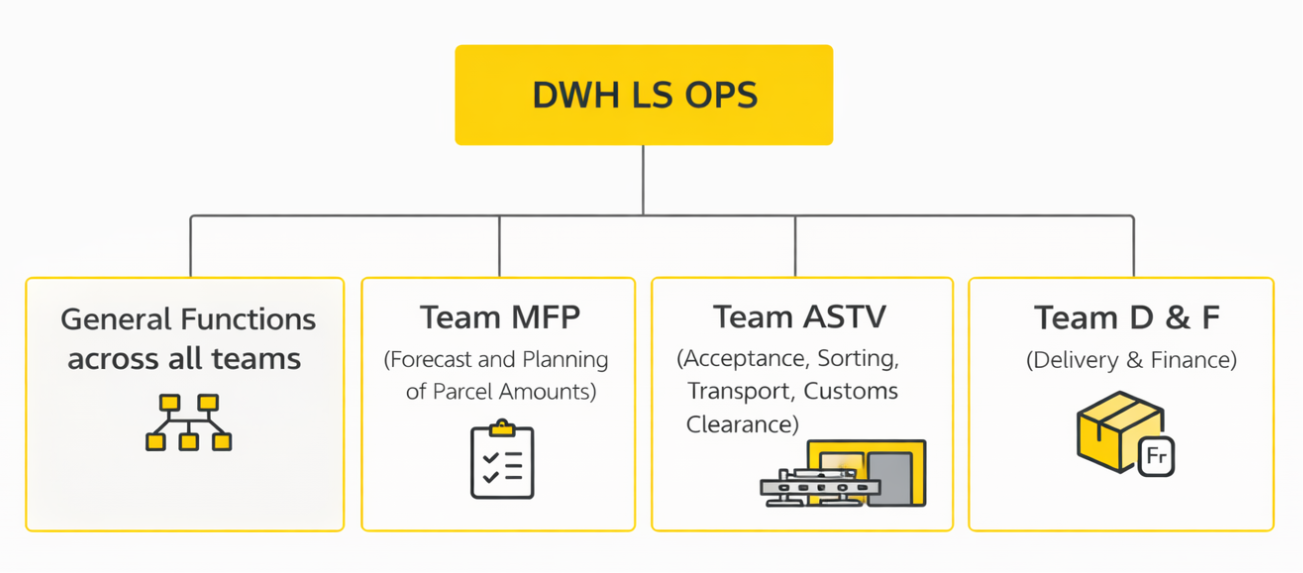
\includegraphics[width=0.8\textwidth]{./content/img/ProjectManagement/BizDevOps_OrgChart.png}
    \caption{Team and sub-team organisation}
    \label{fig:dwhlsops_member_names}
\end{figure}

\subsubsection*{AWS modernisation team}
\label{sec:AWSmodernisationteam}
Swiss Post is currently in a process the modernisation of the AWS cloud environment, which the Swiss Post itself describes as follows:

\textit{Swiss Post is currently pursuing a strategic modernisation of its AWS-based data lake with the objective of improving developer efficiency, increasing operational reliability, and establishing a modern, data-driven architecture. According to internal documentation, the initiative is aligned with defined key performance indicators and aims for completion by the end of the first quarter of 2026 \cite{SwissPostAWSModernization}.}

This modernisation is performed with the assistance of consultants as part of improving AWS usage in DWH LS OPS. The improvements are detailed in 15 \gls{KPI}s across topics such as \gls{AWSGlue} job optimisation and deployment pipeline improvements. With the assistance of the consultants, best practices are applied to the development of \gls{ETL}, as well as general improvements to deployment pipelines. Most importantly for this project, the initiative also includes \gls{DQM} improvements. As a reference, a screenshot of the Confluence landing page describing the initiative is shown below:

\begin{figure}[H]
    \centering
    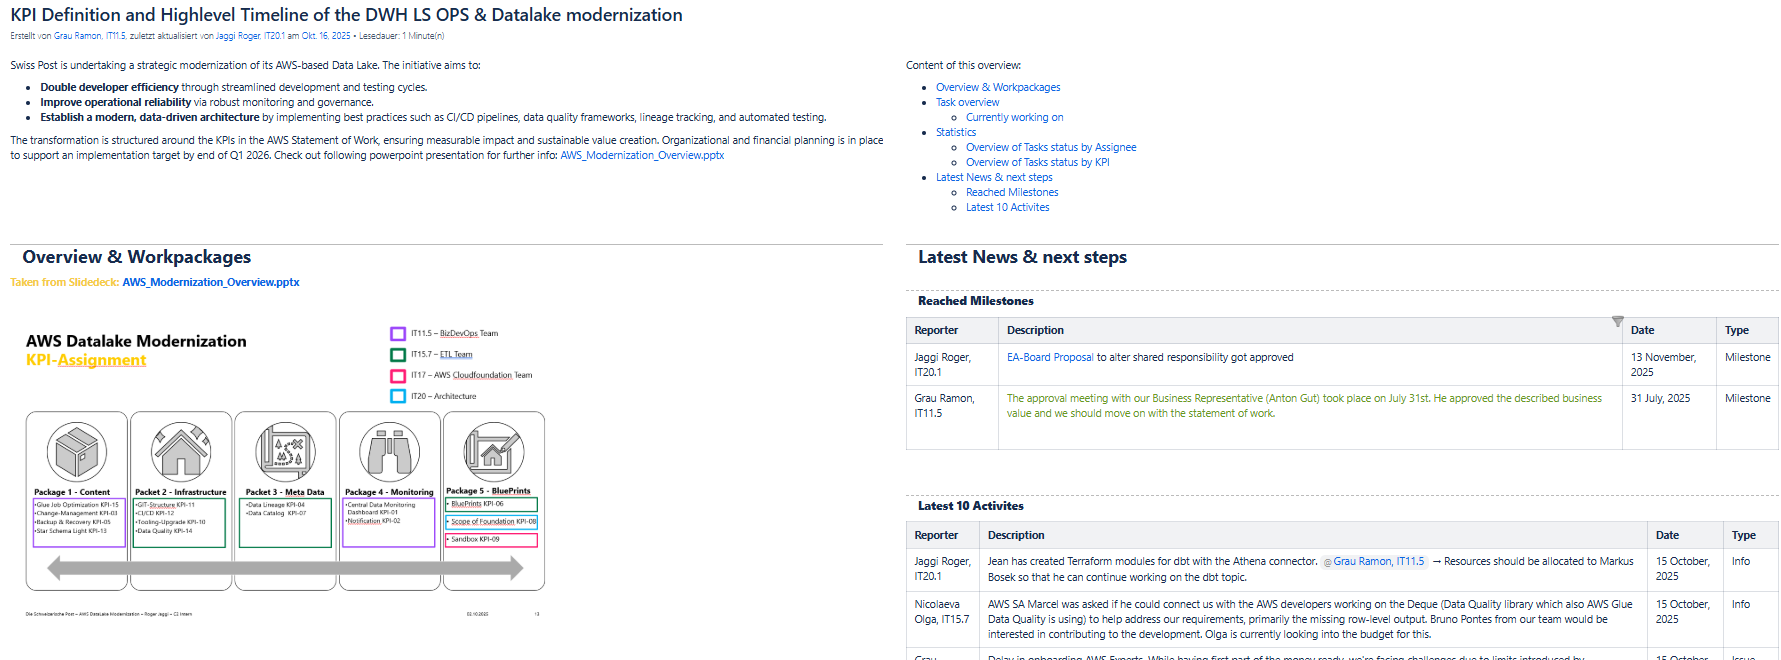
\includegraphics[width=0.8\textwidth]{./content/img/ProjectManagement/AWS_Modernisation_StartPage.png}
    \caption{The start page of the AWS modernisation, listing KPI and latest news}
    \label{fig:aws_modernisation_startpage}
\end{figure}

This team consists mainly of consultants with long-term experience in assisting companies in becoming proficient with AWS. They support data engineers at Swiss Post by improving existing code and reviewing it for potential enhancements. This is relevant for Swiss Post, as the development of the cloud infrastructure started without full architectural support and therefore has room for improvement.

\begin{figure}[H]
    \centering
    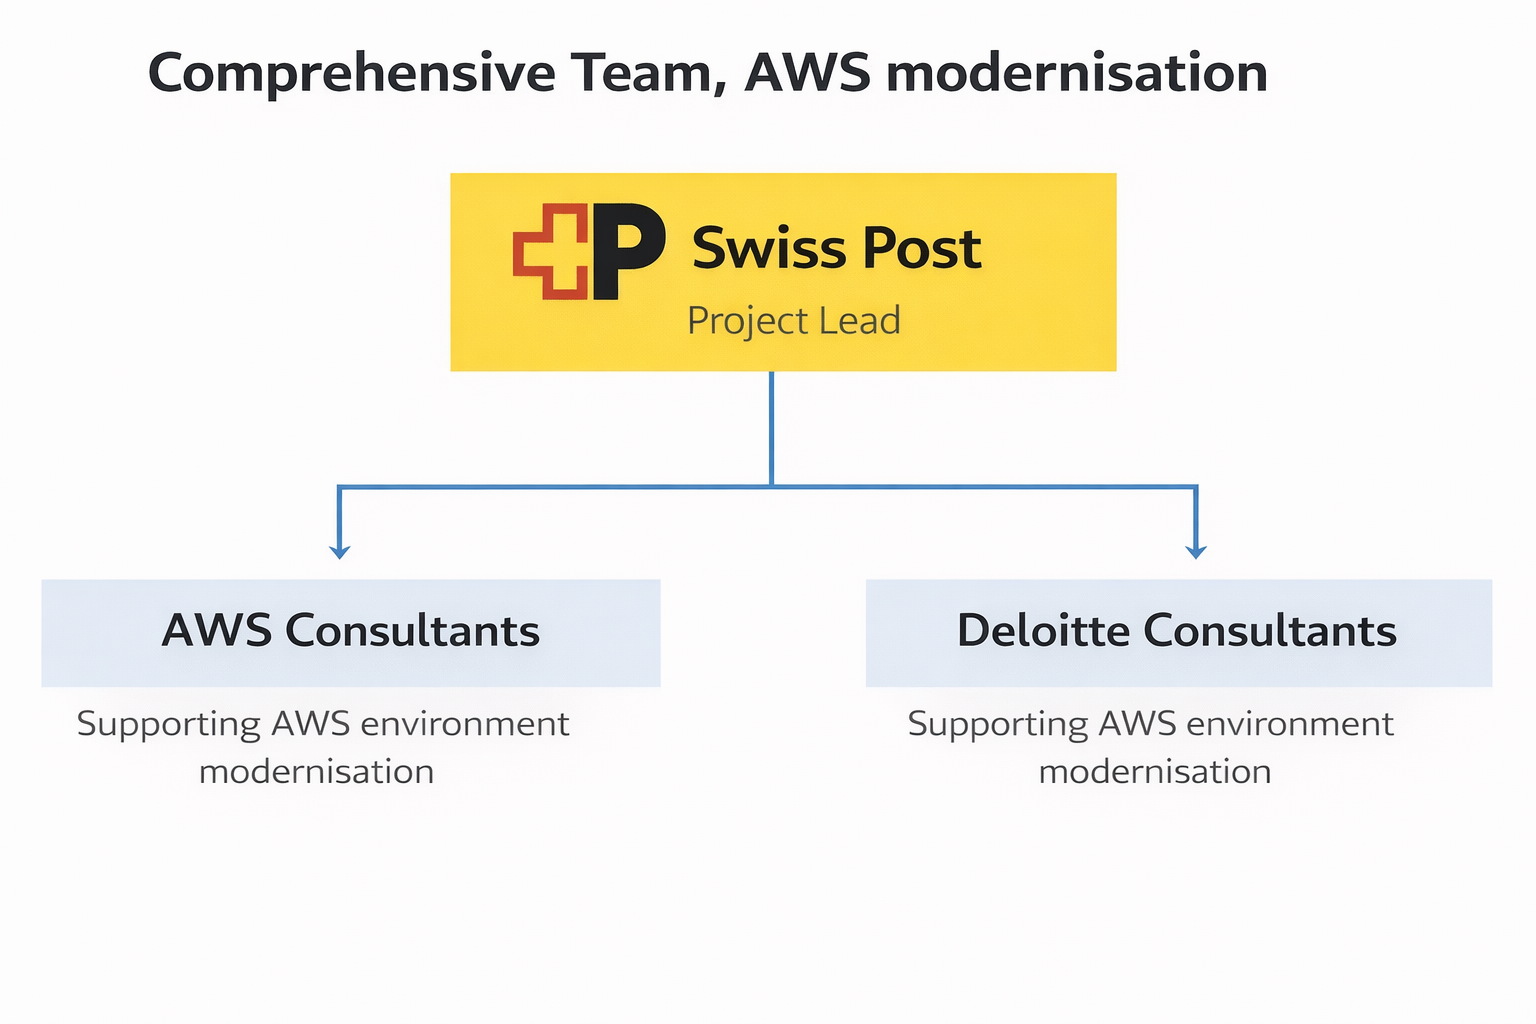
\includegraphics[width=0.8\textwidth]{./content/img/ProjectManagement/AWS_Modernisation_Setup.png}
    \caption{The team setup of the AWS modernisation}
    \label{fig:aws_modernisation_teammembers}
\end{figure}

\subsubsection*{DQM team}
\label{sec:DQMteam}
The third team relevant to the project is the \gls{DQM} team. The team serves KPI 14 Data Quality within the AWS modernisation. Their goal is described on Confluence as follows: specify, review, and implement an MVP to enable data scientists and ETL engineers to forward data quality measures to a monitoring dashboard for both business users and developers.

\begin{figure}[H]
    \centering
    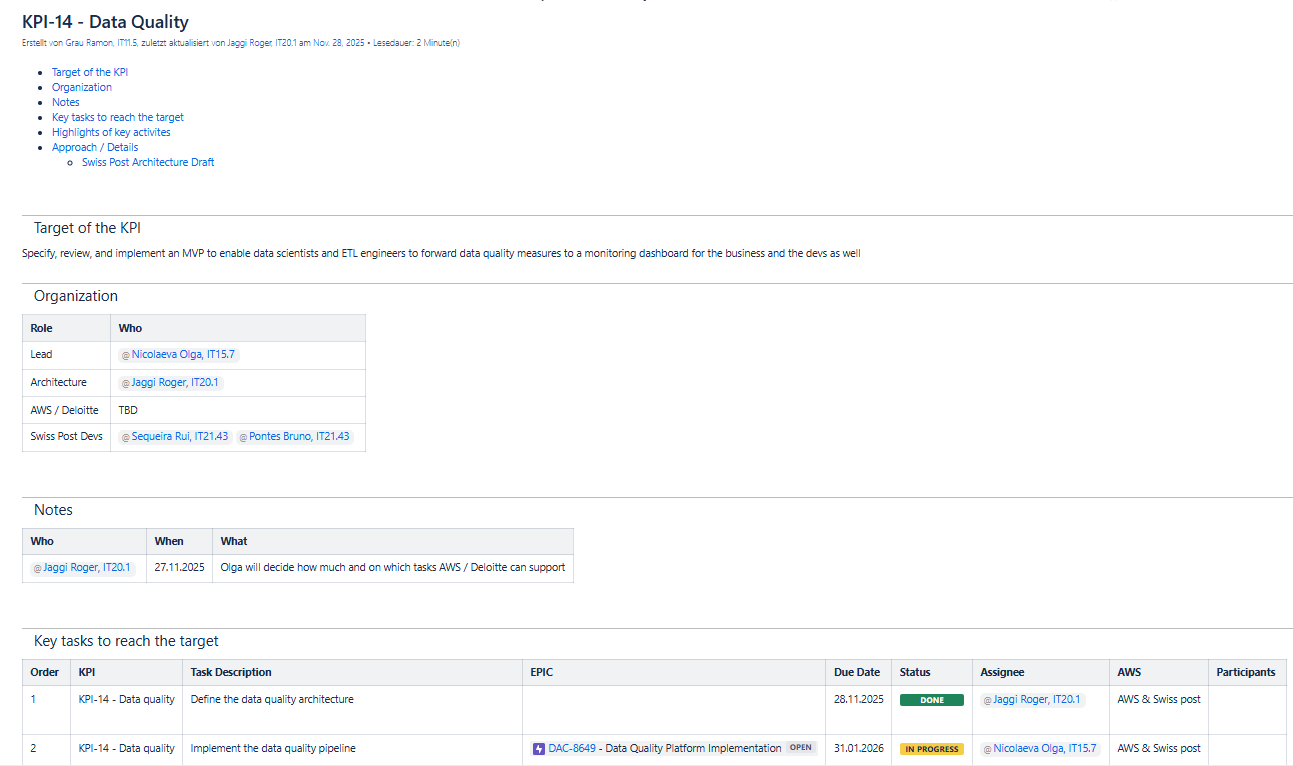
\includegraphics[width=0.8\textwidth]{./content/img/ProjectManagement/Startpage_DQM_KPI14.png}
    \caption{The KPI 14 Data Quality start page on DWH LS OPS Confluence}
    \label{fig:dwhlsops_kpi14_dqm}
\end{figure}

The team consists of three developers with the assistance of a lead data engineer. This setup ensures that the developers can deliver results efficiently, while the lead data engineer provides design guidance and solution structure.

\begin{figure}[H]
    \centering
    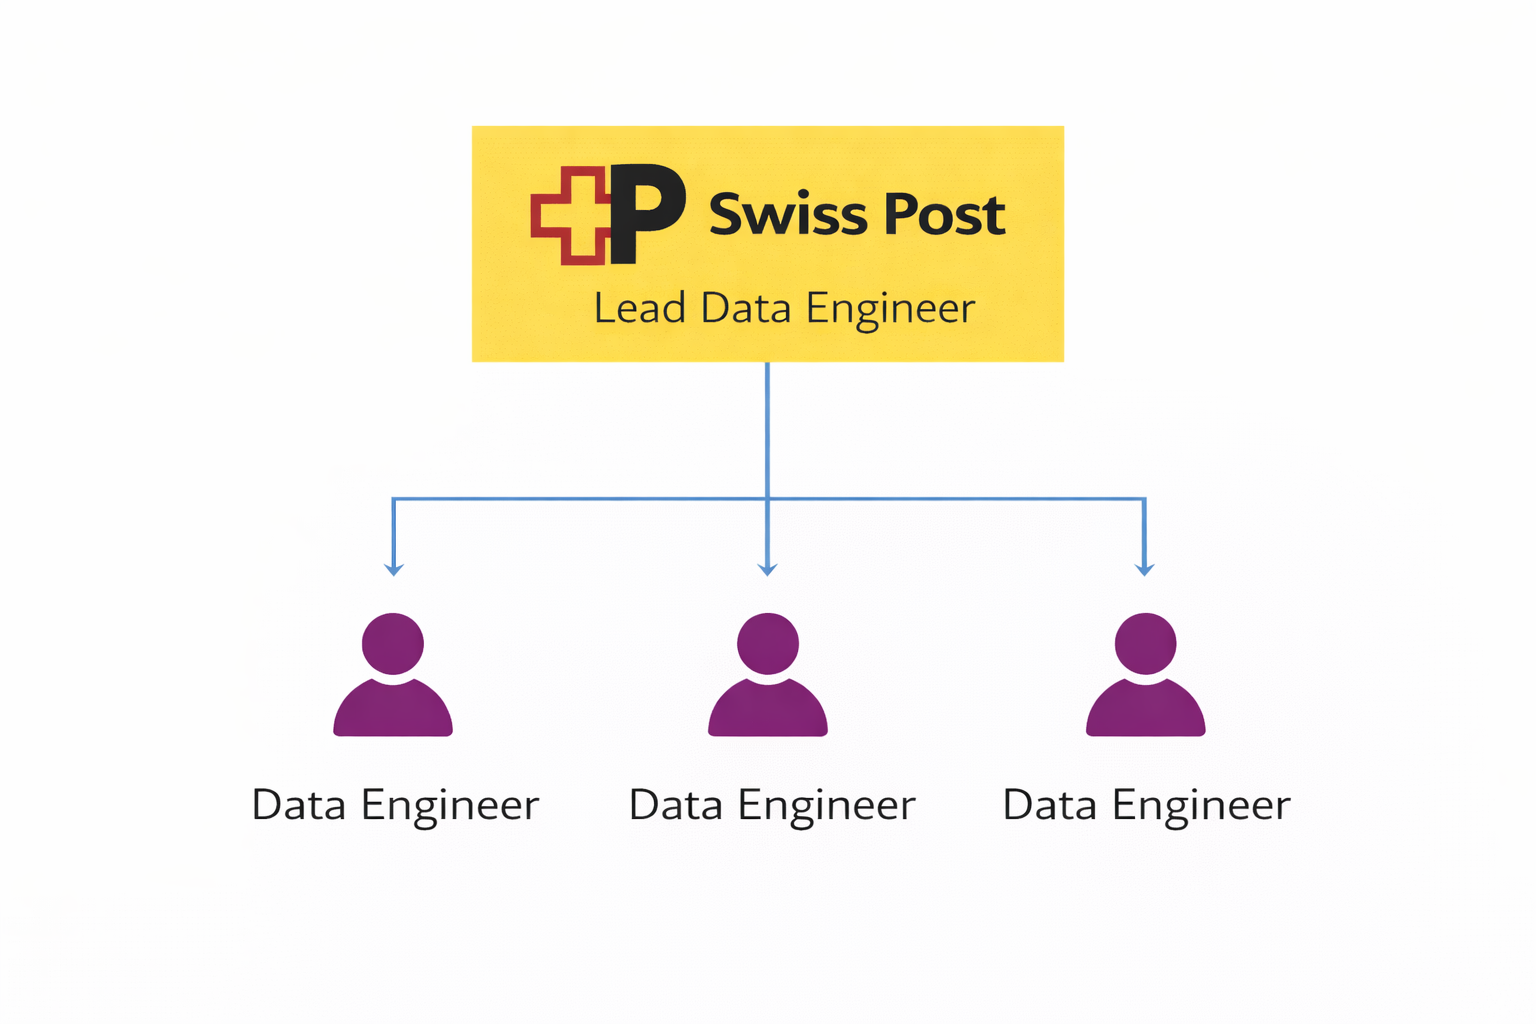
\includegraphics[width=0.8\textwidth]{./content/img/ProjectManagement/DQM_KPI14_Team_NoNames.png}
    \caption{The DQM team setup}
    \label{fig:dwhlsops_kpi14_team_dqm}
\end{figure}

\subsection*{Academic project team}
\label{sec:AcademicTeam}
The academic team consists of the author and the academic advisor. The author conducts the practical work, which includes analysis, implementation, and evaluation. The advisor provides expertise in the academic process and acts as a sparring partner regarding the writing process and project management, offering methodological and academic supervision.

\begin{figure}[H]
    \centering
    
\includegraphics[width=0.8\textwidth]{./content/img/ProjectManagement/ProjectTeam_clean.png}
    \caption{The academic team setup}
    \label{fig:academic_team}
\end{figure}
